\chapter{Implementácia}
\label{implementacia}
\tab V kapitole \ref{porovnanie} boli uvedené rôzne premyselne využívané programy a nástroje na simuláciu a riadenie prevádzky SCADA systémov. V kapitole \ref{bezpecnost} bola popísaná bezpečnosť týchto systémov spolu s rôznymi typmi útokov, ktoré sú pre ne hrozbou. Z nadobudnutých informácií bolo navrhnuté a implementované simulačné prostredie pre protokoly DLMS/COSEM a IEC 104 na testovanie rôznych typov útokov a sledovanie reakcií systému na ne. V nasledujúcej časti bude podrobne popísaná implementácia prostredia spolu s testovaním. \par
\section{Návrh prostredia}
\tab Prvý návrh prostredia pre protokol DLMS/COSEM spočíval vo vytvorení vlastného objektu za pomoci C++ knižnice od spoločnosti GuruX, ktorý sa pripojí do existujúcej siete a bude slúžiť ako zadný vchod (backdoor) do systému. Útoky tohto typu boli popísané v kapitole \ref{bezpecnost}. Avšak s novo-vytvoreným objektom nechcel program DLMS Director spolupracovať a nebolo možné vykonávať testy. Po komunikácií so spoločnosťou GuruX som zistil, že program nepodporuje komunikáciu so špecifickými objektami a v čase písania tejto práce nebol program aktualizovaný o túto funkcionalitu. \par
Druhý návrh, ktorý bol spoločný pre oba skúmané protokoly (DLMS/COSEM a IEC 104) pozostával z vytvorenia programu, ktorý bude simulovať stranu klienta, a bude serveru zasielať nevalidné alebo zmenené príkazy, a budú sa sledovať reakcie systémov. Komunikáciu program nevytvára, iba ďalej zasiela príkazy z odchytenej a následne zmenenej komunikácie. Výhodou je, že pracuje na štvrtej (transportnej) vrstve TCP/IP modelu a vďaka tomu nemusí rozlišovať, s akým protokolom komunikuje. Iba posiela ďalej príkazy ktoré dostane na vstupe, a čaká na odpoveď. Na obrázku \ref{orig} je ukážka validného prostredia, z ktorého sa vychádzalo pri testovaní zmien v príkazoch, ako je možné vidieť na obrázku \ref{test}. Validácia vzorových systémov preukázala, že programy sú schopné simulovať komunikáciu odpovedajúcu štandardom protokolov a je preto možné ich použiť na testovacie účely a očakávať obdobné reakcie aj od reálnych zariadení.
\begin{figure}[h]
    \centering
    \scalebox{0.7}{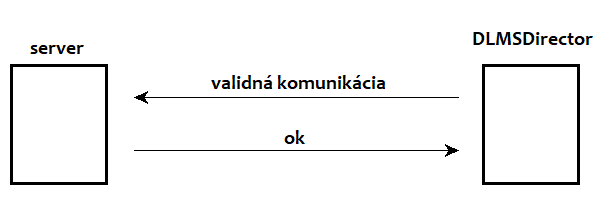
\includegraphics{orig.png}}
    \caption{Vzorový systém}
\label{orig}
\end{figure}
\begin{figure}[h]
    \centering
    \scalebox{0.7}{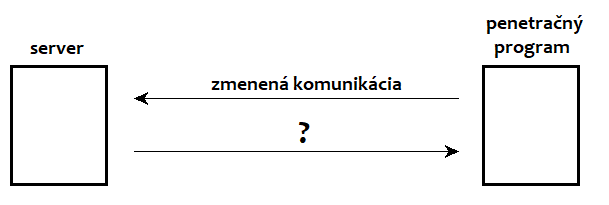
\includegraphics{test.png}}
    \caption{Testovací systém}
\label{test}
\end{figure}
\section{Implementácia simulačného prostredia}
\tab Ako bolo spomenuté vyššie, pre účely simulácie útokov bol vytvorený program klienta, ktorý je schopný zasielať strane servera rôzne zmenené alebo nevalidné príkazy. Program je implementovaný v jazyku C++ a funguje ako TCP klient, ktorý sa pripojí na server. Na vstup dostáva binárny súbor obsahujúci jednotlivé príkazy, ktoré sa budú serveru odosielať. Príkazy boli získané analýzou zachytenej komunikácie medzi reálnymi stanicami klient a server. Analýza prebiehala pomocou nástroja {\tt Wireshark\footnote{Wireshark \url{https://www.wireshark.org}}}. V nástroji bol zobrazený {\tt TCP stream} zachytenej komunikácie a následne odfiltrovaný iba na správy zasielané stranou klienta. Analýza však nemusí prebiehať výhradne pomocou nástroja {\tt Wireshark}. Je možné použiť akýkoľvek obdobný nástroj. Napríklad pre analýzu priamo z príkazovej riadky je možné použiť nástroj {\tt tshark\footnote{TShark \url{https://www.wireshark.org/docs/man-pages/tshark.html}}}, príkazom {\tt tshark -r input.pcap -q -z follow,tcp,raw,0 > output}. Príkaz zobrazí do zadaného súboru binárnu podobu zachytenej komunikácie, ktorú je možné ďalej upravovať. \par
Odfiltrované príkazy boli uložené do binárneho súboru, ktorý sa ďalej posiela ako vstup simulačnému programu. Vďaka tomu, že program pracuje priamo s binárnou podobou príkazov, je možné ich ľubovolne upraviť, a vytvárať so serverom neštandardnú komunikáciu. Odchytenú komunikáciu je možné ďalej analyzovať a zisťovať reakcie systému na rôzne typy útokov. \par
Pri načítavaní jednotlivých príkazov zo súboru je potrebné, aby boli od seba oddelené špecifikým znakom, aby program rozoznal koniec jedného a začiatok druhého. Pôvodne bola zvolená hexadecimálna hodnota {\tt 0x0a}, čo je hodnota pre nový riadok. Túto hodnotu však bolo nutné zmeniť, pretože {\tt 0x0a} sa v jednotlivých príkazoch často vyskytuje aj ako hodnota 10 označujúca objekt alebo namerané dáta. Pri načítavaní to spôsobovalo rozdelenie jedného príkazu na dva. Po tomto zistení som sa pokúšal nájsť inú hexadecimálnu hodnotu ktorá sa nevyskytuje v príkazoch ani jedného z protokolov. Spoločnú hodnotu sa mi nepodarilo nájsť a preto za príkazy protokolu DLMS bola pridaná hodnota {\tt 0x3f} a za príkazy protokolu IEC 104 hodnota {\tt 0x7e}. Príkazy boli upravované v nástroji {\tt Sublime Text 3\footnote{Sublime Text \url{https://www.sublimetext.com}}} po zobrazení hexadecimálneho kódovania. \par 
\subsection{Popis behu programu}
\tab Program pri spustení načíta vstupné argumenty, skontroluje správnosť ich kombinácie a validitu zadaných hodnôt. Keď je všetko v poriadku, zo vstupu sa načítajú jednotlivé príkazy, ktoré sa budú odosielať. Pri spustení programu je potrebné zadať, s akým protokolom má program pracovať, DLMS alebo IEC 104. Je to nutné z dôvodu, že program rozlišuje podľa akého znaku má jednotlivé príkazy od seba odlíšiť, ako už bolo spomínané vyššie. Protokol DLMS/COSEM taktiež využíva na prenos príkazov protokol HDLC, ktorý slúži na spoľahlivý prenos dát po sieti. Súčasťou dátového rámca protokolu sú dva byty vyhradené na tzv. kontrolný súčet CCITT-CRC16. Ukážka rámca je na obrázku \ref{hdlc}. Príkazy protokolu DLMS obsahujú prvý a posledný byte režijný, označujúci začiatok a koniec príkazu, hodnota je {\tt 0x7e}. Následuje adresa, typ príkazu, samotné data a dva byty s hodnotou spomínaného kontrolného súčtu. 
\begin{figure}[h]
    \centering
    \scalebox{0.5}{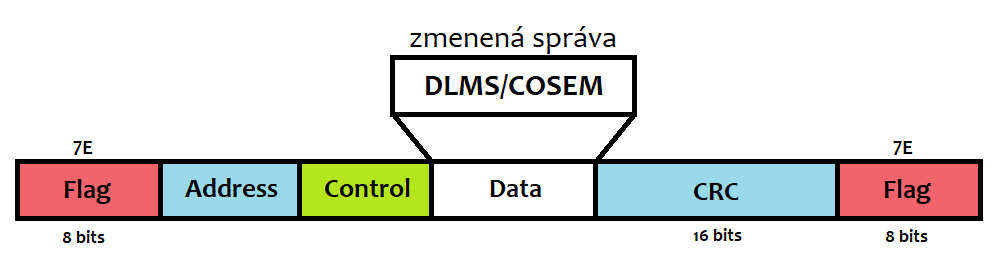
\includegraphics{hdlc.png}}
    \caption{HDLC zapúzdrenie}
\label{hdlc}
\end{figure}
Pre každý zmenený príkaz je potrebné nanovo vypočítať jeho kontrolný súčet. Ten sa počíta z celého rámca, okrem prvého a posledného (režijného bytu). Ak by totiž súčet nesúhlasil s dátami, strana príjemcu (servera) by správu zahodila a prestala by ďalej komunikovať. Implementácia funkcií na výpočet súčtu bola prevzatá zo stránok {\tt stackoverflow.com}\footnote{Stackoverflow \url{https://stackoverflow.com/questions/7983862/calculating-fcscrc-for-hdlc-frame} [Online: Marec 2018]} a {\tt www.zorc.breitbandkatze.de}\footnote{CRC \url{http://www.zorc.breitbandkatze.de/crc.html} [Online: Marec 2018]}. Program načítava jednotlivé príkazy do pomocnej premennej {\tt message} typu {\tt std::vector<std::string>}. Do premennej {\tt answer}, ktorá je rovnakého typu sa ukladajú odpovede od servera. \par
Po načítaní jednotlivých príkazov sa vytvorí TCP spojenie a začína komunikácia. Príkazy sa odosielajú v cykle. Pre protokol DLMS sa vždy odošle jeden príkaz a očakáva sa jedna odpoveď, nakoľko protokol komunikuje synchrónne. Protokol IEC104 je o niečo komplikovanejší. Oproti protokolu DLMS, kde ide o synchrónnu komunikáciu 1:1 (jedna správa : jedna odpoveď), to tak pri protokole IEC 104 nefunguje, komunikácia prebieha asynchrónne. Niekedy je potrebné odoslať niekoľko správ bez odpovedi, alebo očakávať niekoľko odpovedí po jednej správe. Problém bol vyriešený využitím funkcie {\tt select()} spolu s {\tt timeoutom}. Funkcia je volaná v cykle. Ak sa podarí prijať správu, cyklus prijímania sa opakuje, ak vyprší timeout, z cyklu sa vyskočí a odosiela sa nová správa.
Komunikácia je implementovaná pomocou {\tt bsd schránok}. Odosielanie a prijímanie správ zabezpečujú funkcie {\tt send()} a {\tt recv()}. 
\subsection{Návod na použitie}
\subsubsection{Preloženie a spustenie programu}
Program je nutné pred prvým spustením preložiť príkazom {\tt make} v koreňovom adresári projektu. Keď je program preložený, môžeme ho spustiť. Spúšťa sa nasledovným príkazom: \newline
{\tt ./client [-h] [a <adresa serveru>] [-p port] [-i vstupný súbor] [-o výstupný súbor] [--dlms] [--iec]}
\subsubsection{Parametre programu}
Program {\tt client} je možné spustiť s niekoľkými parametrami:
\begin{description}
\item {\tt -h \textendash\textendash help} - zobrazí nápovedu
\item {\tt -a \textendash\textendash address} - IP adresa serveru, s ktorým bude klient komunikovať
\item {\tt -p \textendash\textendash port} - port, na ktorom komunikuje server
\item {\tt -i \textendash\textendash input} - vstupný binárny súbor s jednotlivými príkazmi
\item {\tt -o \textendash\textendash output} - súbor, kam sa budú ukladať odpovede od serveru
\item {\tt -1 \textendash\textendash iec} - komunikácia s iec 104 serverom
\item {\tt -2 \textendash\textendash dlms} - komunikácia s dlms serverom
\end{description}
Vždy musí byť zadaný aspoň jeden z parametrov {\tt -h \textendash\textendash help}, {\tt -a \textendash\textendash address} | {\tt \textendash\textendash dlms}, {\tt -o \textendash\textendash output}. Nemôžu byť zadané oba naraz, ani z jednej kombinácie. Navyše parameter {\tt -h \textendash\textendash help} nemôže byť kombinovaný so žiadnym ďalším parametrom. Pri absencií parametra {\tt -p \textendash\textendash port} sa nastaví predvolená hodnota podľa zadaného protokolu. {\tt 2404} pre IEC 104 a {\tt 4059} pre DLMS. V prípade nezadanie parametrov {\tt -i \textendash\textendash input} a {\tt -o \textendash\textendash output} sa využije štandardný vstup a výstup.
\subsubsection{Príklady použitia}
\begin{description}
\item {\tt ./client -h} - vypíše nápovedu
\item {\tt ./client -a 192.168.137.189 -p 4060 \textendash\textendash dlms -i data1 -o output1} - program bude komunikovať s DLMS serverom na porte 4060 pomocou protokolu TCP. Príkazy si načíta zo súboru {\tt data1} a odpovede od servera zapíše do súboru {\tt output1}. Ak takýto súbor neexistuje, vytvorí ho.
\end{description}
\section{Testovanie}
\tab Pri validácií programu klienta a simulačného prostredia ako takého boli využívané zachytené komunikácie medzi jednotlivými simulátormi SCADA prevádzky. Zachytená komunikácia bola v simulačnom prostredí opätovne vytvorená a zachytená. Po overení, že všetky dvojice komunikácií sú totožné, bol program prehlásený za validný. \par
\begin{figure}[h]
    \centering
    \scalebox{0.5}{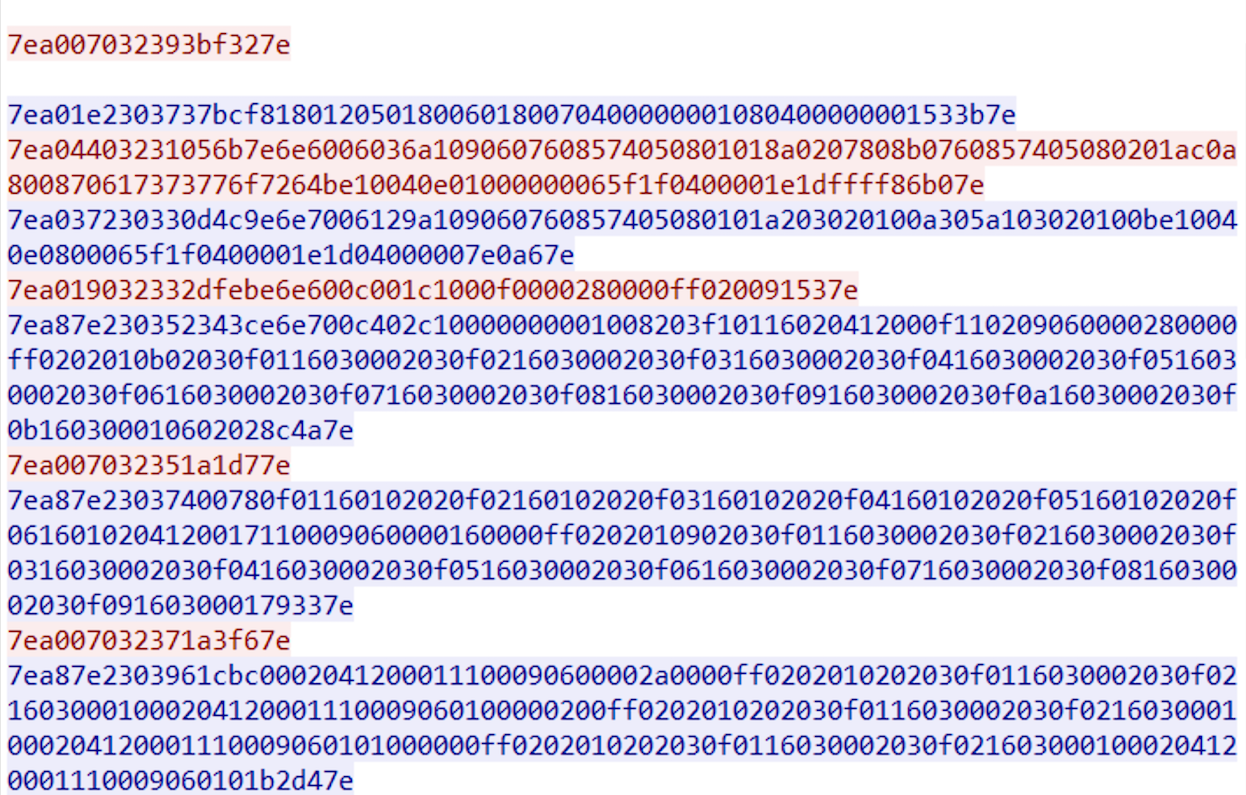
\includegraphics{original}}
    \caption{Originálna komunikácia medzi klientom a serverom}
    \label{original}
\end{figure}
Na obrázku \ref{original} je ukážka časti zachytenej originálnej komunikácie medzi simulačnými nástrojmi pre klienta a server, konkrétne ide o protokol DLMS/COSEM. Na obrázku \ref{testing} je možné vidieť tú istú komunikáciu vygenerovanú pomocou simulačného programu klienta. Obe komunikácie boli následne porovnané programom {\tt diffchecker\footnote{Diffchecker \url{https://www.diffchecker.com} [Online: Marec 2018]}} a bolo overené, že komunikácie sú totožné. \par
\begin{figure}[h]
    \centering
    \scalebox{0.5}{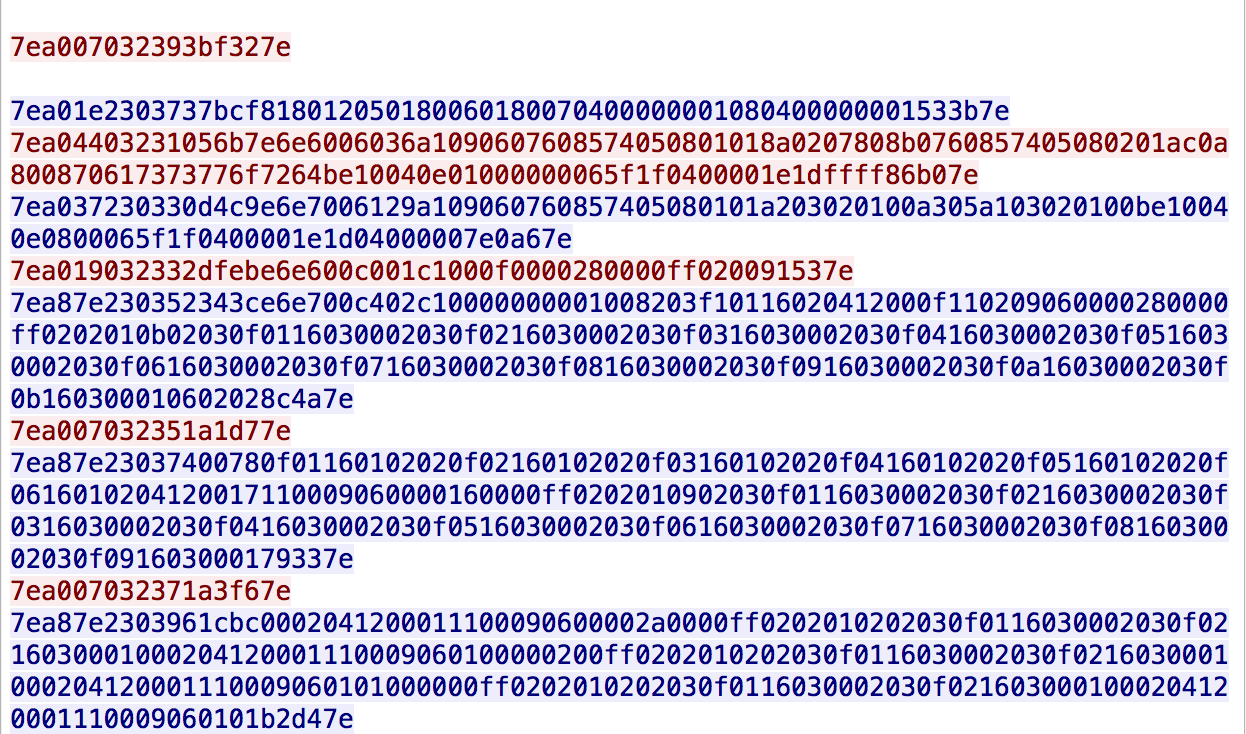
\includegraphics{testing}}
    \caption{Opätovne vygenerovaná komunikácia pomocou programu klienta}
    \label{testing}
\end{figure}
Pri testovaní protokolov bola vždy vytvorená testovacia topológia so vzorovou komunikáciou. Komunikácia bola pri každom teste čiastočne zmenená a boli sledované reakcie systému, ako je možné vidieť na obrázku \ref{monitoring}. \par
\begin{figure}[h]
    \centering
    \scalebox{0.8}{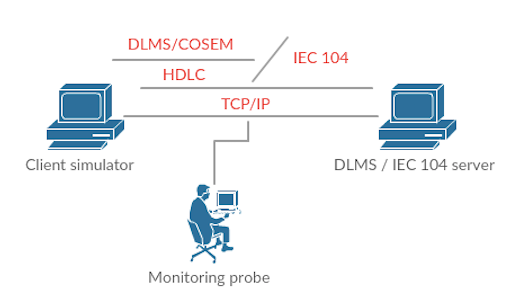
\includegraphics{monitoring}}
    \caption{Sledovanie reakcií systému zo zachytenej komunikácie}
    \label{monitoring}
\end{figure}
Pri testovaní bezpečnostných incidentov na systémy komunikujúce pomocou protokolov DLMS/COSEM a IEC 104 som postupoval v niekoľkých krokoch:
\begin{enumerate}
\item Vytvorenie simulačného prostredia, ktoré sa chová ako reálny systém.
\item Vygenerovanie validnej komunikácie, ktorá bude slúžiť ako vzorová.
\item Pozmenenie príkazov z ochytenej vzorovej komunikácie.
\item Opätovné vygenerovanie s patričnými zmenami.
\item Sledovanie reakcií systému.
\end{enumerate}

\subsection{DLMS/COSEM}
\tab Pri testovaní protokolu DLMS bola využívaná open source knižnica pre jazyk C++ poskytovaná spoločnosťou GuruX. Knižnica je voľne dostupná v Github repozitári\footnote{DLMS knižnica - Github \url{https://github.com/Gurux/Gurux.DLMS.cpp} [Online: Marec 2018]}. Podrobná inštalácia knižnice je popísaná medzi prílohami v časti \ref{kniznica}. Knižnica obsahuje vzorový program pre server, ktorý bol následné upravený pre potreby testovania. Pôvodná implementácia zahŕňa štyry rôzne typy DLMS serverov, pričom každý komunikuje na inom porte. \par
Pri testovaní bol ponechaný iba jeden server využívajúci logické mená (Logical Names), komunikujúci na porte 4060. Taktiež bola povolená možnosť hodnoty v atribútoch jednotlivých objektov aj nastavovať. Pôvodne ich bolo možné iba vzdialene čítať. Čo sa týka knižnice samotnej, implementácia dátových objektov nepodporovala dynamickú zmenu nameraných hodnôt za behu programu. Aby to viac odpovedalo reálnemu systému, v súbore {\tt GXDLMSData.cpp} bola zmenená implementácia {\tt CGXDLMSData::GetValue} metódy, ktorá vracala nameranú hodnotu. Do metódy bola pridaná podmienka, ktorá vráti novú hodnotu ak od predošlého dotazu uplynulo aspoň 10 sekúnd. Uplynutý čas od posledného dotazu sa počíta pomocou premennej typu {\tt std::time\_t}, pričom sa počíta rozdiel jej hodnoty (od posledného dotazu) k aktuálnemu času {\tt std::time(nullptr)}. Nové hodnoty sa získavajú dvoma spôsobmi. Sú generované náhodne funkciou {\tt rand()} alebo sú načítavané zo súboru. Voľba konkrétneho spôsobu je na základe konfiguračného súboru, ktorý je uložený v {\tt Gurux.DLMS.cpp-master/conf}. Obsah konfiguračného súboru môže byť napríklad:
\begin{itemize}
\item {\tt file = ../../values} - nastavenie čítania zo súboru {\tt values} spolu s cestou k nemu
\item {\tt rand = 1000} - nastavenie náhodného generovania hodnôt z rozsahu 0..1000
\end{itemize} \par
\begin{figure}[h]
    \centering
    \scalebox{0.4}{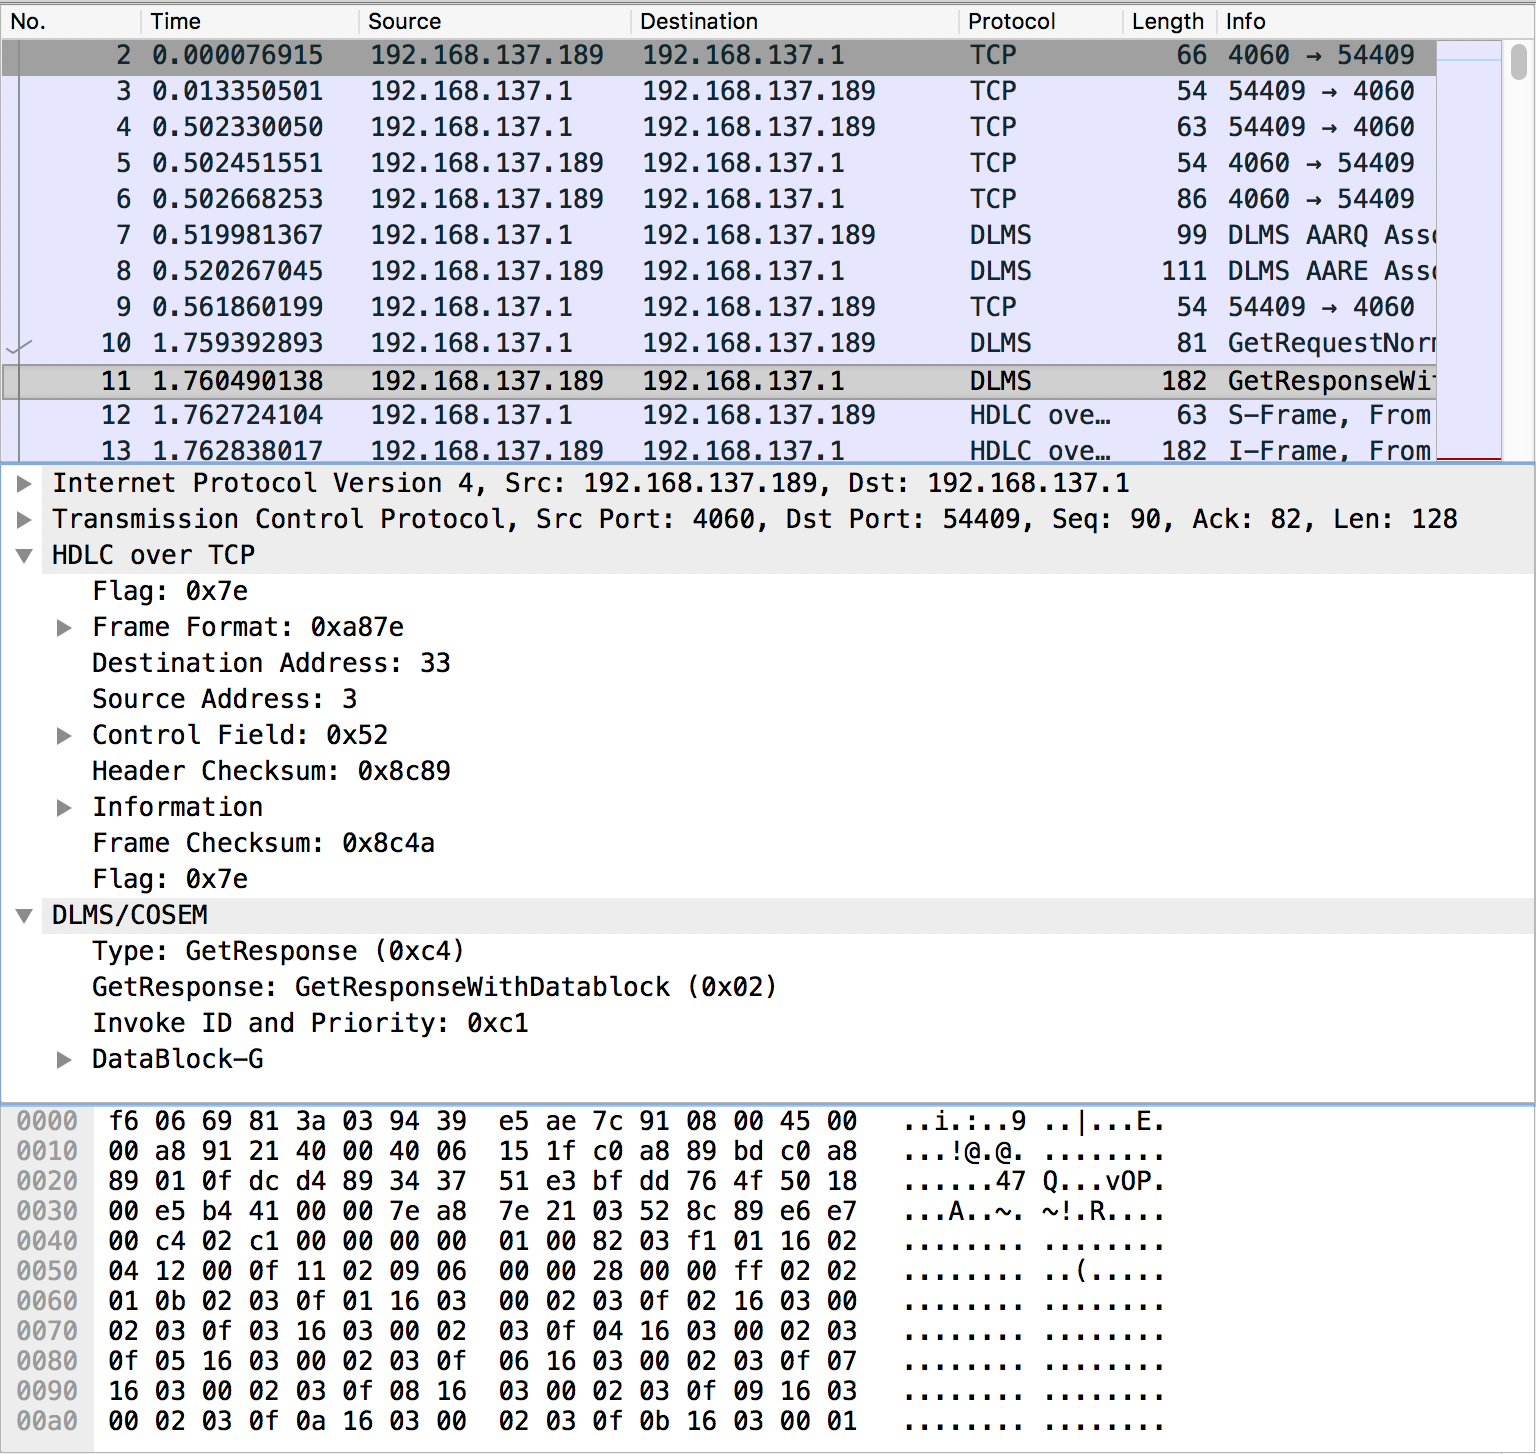
\includegraphics{dissector}}
    \caption{Analýza zachytenej komunikácie}
    \label{dissector}
\end{figure}
Pri analýze zachytených .pcap súborov bol použitý dissector pre program Wireshark vytvorený pánom Ing. Petrom Matouškom, Ph.D., M.A.\footnote{DLMS Dissector \url{https://github.com/matousp/dlms-analysis} [Online: Apríl 2018]} Dissector z načítanej binárnej postupnosti vyberie časti pre HDLC zapúzdrenie a pre samotné dáta protokolu DLMS/COSEM. Ukážku je možné vidieť na obrázku \ref{dissector}.
\subsubsection{Testy}
\subsubsection{Validná komunikácia:} 
Na začiatku testovania bol vytvorený vzorový .pcap súbor obsahujúci validnú (vzorovú) komunikáciu protokolu DLMS/COSEM. Zasielané príkazy boli následne systematicky menené a boli sledované reakcie systému. \par
\noindent \textbf{Zachytenie komunikácie:} dlms.pcap
\subsubsection{Test č. 1:}
\textbf{Zmena:} Data obsahovali zlú veľkosť pri otváraní asociácie v príkaze {\tt AARQ - Association Request}. 11 bytov namiesto 9 bytov: 0x09 $\rightarrow$ 0x0b. \newline
\textbf{Reakcia:} Server si zmenu vôbec nevšímal a zaslal spätne potvrdzovaciu správu o zistení deviatich pripojených zariadení. \par
\noindent \textbf{Zachytenie komunikácie:} data1.pcap
\subsubsection{Test č. 2:}
\textbf{Zmena:} Dĺžka OID prvého požiadavku bola zle zadaná v príkaze {\tt AARQ - Association Request}. 9 bytov namiesto 7 bytov: 0x07 $\rightarrow$ 0x09. \newline
\textbf{Reakcia:} Server si opäť zmenu nevšimol. Žiadosť o asociáciu prijal a odpoveď obsahovala OID zmenené na správne. \par
\noindent \textbf{Zachytenie komunikácie:} data2.pcap
\subsubsection{Test č. 3:}
\textbf{Zmena:} Dĺžka OID prvého požiadavku bola zle zadaná v príkaze {\tt AARQ - Association Request}. 3 byty namiesto 7 bytov: 0x07 $\rightarrow$ 0x03. \newline
\textbf{Reakcia:} Reakcia bola rovnaká ako pri predchádzajúcom teste. \par
\noindent \textbf{Zachytenie komunikácie:} data3.pcap
\subsubsection{Test č. 4:}
\textbf{Zmena:} Zlý typ paketu. Pôvodná správa bola typu {\tt Get-Request} a bola následne zmenená na {\tt Set\--Request}: 0xc0 $\rightarrow$ 0xc1. Zmena bola vykonaná iba v poli obsahujúcom typ. Zvyšok paketu ostal pôvodný pre {\tt Get-Request}. \newline
\textbf{Reakcia:} Server prijal žiadosť na nastavenie hodnoty, vykonal zmenu a odpovedal potvrdzovacou správou o úspešnom nastavení. \par
\noindent \textbf{Zachytenie komunikácie:} data4.pcap
\subsubsection{Test č. 5:}
\textbf{Zmena:} Zlý typ paketu. Namiesto {\tt Get-Request} sa poslalo {\tt Set-Response}: 0xc0 $\rightarrow$ 0xc5. \newline
\textbf{Reakcia:} Server nevedel, ako má zareagovať a na správu neodpovedal. \par
\noindent \textbf{Zachytenie komunikácie:} data5.pcap
\subsubsection{Test č. 6:}
\textbf{Zmena:} Chybný OBIS kód požadovaného objektu. Požaduje sa 0.0.40.0.0.1 namiesto 0.0.40.0.0.255: 0xff $\rightarrow$ 0x01. \newline
\textbf{Reakcia:} Server žiadosť prijal a pokúsil sa vrátiť požadovanú odpoveď. Odoslal ale prázdnu správu, nakoľko požadovaný objekt nepoznal. \par
\noindent \textbf{Zachytenie komunikácie:} data6.pcap
\subsubsection{Test č. 7:}
\textbf{Zmena:} Zmena požadovaného atribútu objektu. Požaduje sa atribút 10 namiesto 1: 0x02 $\rightarrow$ 0x0a. \newline
\textbf{Reakcia:} Server na zmenu reagoval štandardnou odpoveďou a vrátil hodnotu požadovaného atribútu. Tento test bol zameraný skôr na typ útoku, kedy útočník zachytí prebiehajúcu komunikáciu, čiastočne zmení obsah príkazu, ale ponechá ho validný a pošle pô\-vod\-né\-mu adresátovi. Server správu príjme a odpovie, ale riadiacej stanici príde iná odpoveď akú požadovala. Ak nie je odpoveď dostatočne overená, že je to naozaj tá, ktorá bola očakávaná, môže to znamenať napríklad zlú informovanosť o nameraných hodnotách. \par
\noindent \textbf{Zachytenie komunikácie:} data7.pcap
\subsubsection{Test č. 8:}
\textbf{Zmena:} Zasielané správy odpovedali správam z testovacej komunikácie pre protokol DLMSDirector (DLMSDirector.pcap). Test sa zameriaval na sledovanie otvorenia spojenia a testovanie autentizácie. Komunikácia bola analyzovaná v nástroji {\tt Wireshark}, kde bolo sledované v akej podobe sa prenášajú autentizačné údaje po sieti. \newline
\textbf{Reakcia:} Testovanie autentizácie bolo zamerané hlavne na sledovanie prebiehajúcej komunikácie. Bolo overené, že autentizačné kľúče sa prenášajú v otvorenej podobe. Útočník si tak môže jednoducho ochytiť komunikáciu, prečítať si kľúč a vytvoriť svoje vlastné spojenie so systémom. \par
\noindent \textbf{Zachytenie komunikácie:} auth.pcap \newline \par
Testovanie preukázalo, že server sa pokúša na príkaz vždy odpovedať nehľadiac na to, či požadovaný objekt alebo atribút pozná. Spojenie ukončuje iba v prípade nevalidného príkazu. Veľmi nebezpečný je tiež nešifrovaný prenos hesla po sieti, čo umožňuje útočníkom jednoduchý prístup k autentizačným údajom systému.
\subsection{IEC 104}
\tab Pri testovaní protokolu IEC 104 bol využívaný program QTester 104 a IEC 60870-5-104 Server Simulator. Testovacia topológia pozostávala z jedného klienta a jedného servera, ku ktorému bolo pripojených päť objektov typu {\tt Measured Short Float}. Objekty slúžia na ukladanie nameraných hodnôt s pohyblivou rádovou čiarkou. Testovaciu topológiu je možné vidieť na obrázku \ref{iec-testing}.
\begin{figure}[h]
    \centering
    \scalebox{0.8}{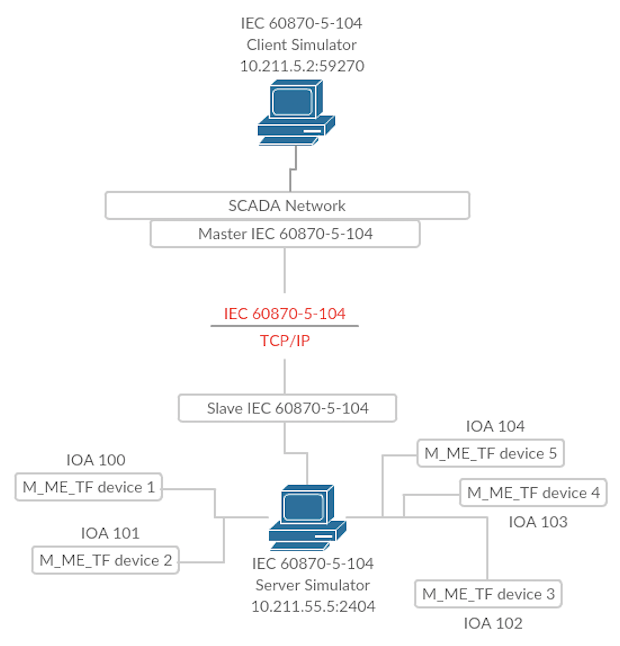
\includegraphics{iec-testing}}
    \caption{Testovacia topológia pre protokol IEC 104}
\label{iec-testing}
\end{figure}
Testovanie protokolu IEC 104 bolo o niečo náročnejšie ako pri protokole DLMS/COSEM z niekoľkých dôvodov. Simulačné programy neumožňovali pridať automatizáciu zmien nameraných hodnôt, a tak bolo potrebné všetky zmeny vykonávať ručne. Z rovnakého dôvodu simulačné prostredie neodpovedalo reálnemu systému do takej miery ako pri DLMS/COSEM. Asynchrónny charakter protokolu tiež trochu skomplikoval opätovné generovanie komunikácie z už odchytenej, ako bolo spomínané vyššie. Posledný problém, ktorý som mal oproti protokolu DLMS/COSEM, bol, že nebolo možné pridať autentizáciu na server a preto ju nebolo možné ani testovať.
\subsubsection{Testy}
\subsubsection{Validná komunikácia:} 
Na začiatku testovania bol vytvorený vzorový .pcap súbor obsahujúci validnú (vzorovú) komunikáciu protokolu IEC 104. Zasielané príkazy boli následne systematicky menené a boli sledované reakcie systému. \par
\noindent \textbf{Zachytenie komunikácie:} iec104.pcap
\subsubsection{Test č. 1:}
\textbf{Zmena:} Test na buffer overflow. Pri nastavovaní hodnoty príkazom {\tt Set point command} bola v poli {\tt Value} zmenená hodnota z 2 na NaN: 0x40 $\rightarrow$ 0xff ffff fff. \newline
\textbf{Reakcia:} Hodnota bola nad rámec povoleného maxima a spôsobila, že dĺžka príkazu bola väčšia ako je štandard, čo spôsobilo, že príkaz bol nevalidný. Server odpovedal hláškou {\tt ERR prefix 1 bytes} spolu s informáciou, že hodnota bola nastavovaná na {\tt nan - Not-A-Number} hodnotu. \par
\noindent \textbf{Zachytenie komunikácie:} data\_buffer\_overflow.pcap
\subsubsection{Test č. 2:}
\textbf{Zmena:} Test na zmenu adresy objektu. Pri nastavovaní hodnoty príkazom {\tt Set point command} bola v poli {\tt Addr} zmenená hodnota adresy cieleného objektu z 1 na 65281: 0x0100 $\rightarrow$ 0x01ff. \newline
\textbf{Reakcia:} Server si zmenu všimol a nevedel nájsť dotazovaný objekt. Odpovedal správou {\tt UkComAdrASDU\_NEGA}. \par
\noindent \textbf{Zachytenie komunikácie:} data\_wrong\_addr.pcap
\subsubsection{Test č. 3:}
\textbf{Zmena:} Test na zmenu dôvodu prenosu. Pri nastavovaní hodnoty príkazom {\tt Set point command} bola v poli {\tt CauseTx} zmenená hodnota z 6 na 10: 0x06 $\rightarrow$ 0x0a (Act (6) na ActTerm (10)). \newline
\textbf{Reakcia:} Server si zmenu všimol a odpovedal správou {\tt UkCauseTx\_NEGA}. \par
\noindent \textbf{Zachytenie komunikácie:} data\_wrong\_cause.pcap
\subsubsection{Test č. 4:}
\textbf{Zmena:} Test na zmenu IOA adresy. Pri nastavovaní hodnoty príkazom {\tt Set point command} bola v poli {\tt IOA} zmenená hodnota z 11 na 15: 0x0b $\rightarrow$ 0x0f. \newline
\textbf{Reakcia:} Server si zmenu všimol a dotazovaný objekt nepoznal. Odpovedal správou {\tt UkIOA\_NEGA}. \par
\noindent \textbf{Zachytenie komunikácie:} data\_wrong\_ioa15.pcap
\subsubsection{Test č. 5:}
\textbf{Zmena:} Test na zmenu OA adresy. Pri nastavovaní hodnoty príkazom {\tt Set point command} bola v poli {\tt OA} zmenená hodnota z 2 na 5: 0x02 $\rightarrow$ 0x05. \newline
\textbf{Reakcia:} Server si zmenu nevšímal a odpovedal potvrdzovacou správou o úspešnom nastavení hodnoty. \par
\noindent \textbf{Zachytenie komunikácie:} data\_wrong\_oa.pcap
\subsubsection{Test č. 6:}
\textbf{Zmena:} Test na zmenu typu id príkazu. Pôvodný príkaz na nastavenie hodnoty - {\tt Set point command} typu {\tt C\_SE\_NC\_1} bol zmenený na typ {\tt C\_BO\_NA\_1 - Bitstring of 32 bits}. Zmena bola vykonaná v poli {\tt TypeId} z hodnoty 50 na hodnotu 51: 0x32 $\rightarrow$ 0x33. Zvyšok príkazu zostal pôvodný pre príkaz typu {\tt C\_SE\_NC\_1}. \newline
\textbf{Reakcia:} Server si zmenu všimol a odpovedal správou {\tt UkIOA\_NEGA}. \par
\noindent \textbf{Zachytenie komunikácie:} data\_wrong\_type\_id.pcap
\subsubsection{Test č. 7:}
\textbf{Zmena:} Posledný test bol opäť nameraný na zmenu hodnoty IOA adresy. Pri nastavovaní hodnoty príkazom {\tt Set point command} bola v poli {\tt IOA} zmenená hodnota z 11 na 12: 0x0b $\rightarrow$ 0x0c. \newline
\textbf{Reakcia:} Server zmenu prijal, cielený objekt našiel medzi pripojenými a odpovedal potvrdzovacou správou o úspešnom nastavení hodnoty. \par
\noindent \textbf{Zachytenie komunikácie:} different\_ioa.pcap \newline









